\documentclass[10pt]{jsarticle}
\usepackage[margin=15truemm]{geometry}
\usepackage[dvipdfmx]{graphicx}
\usepackage{ascmac} % for screen
\usepackage{subfigure} % for subfigure
\usepackage{multicol}
\usepackage{amsmath}
\usepackage{mathtools}
\usepackage{amssymb}
\usepackage{multicol}
\usepackage{tikz}
\usetikzlibrary{intersections, calc, arrows.meta}
\usepackage{wrapfig}
\usepackage{setspace}

\renewcommand{\thesubsubsection}{(\arabic{subsubsection})}


\begin{document}
\section{計算}
\subsection{二次式の展開}
\begin{itembox}[l]{展開の公式}
	\begin{Large}
		\begin{itemize}
			\item $(x+a)^2=$
			\item $(x-a)^2=$
			\item $(x+a)(x-a)=$
			\item $(x+a)(x+b)=$
		\end{itemize}
	\end{Large}
\end{itembox}

\begin{itembox}[l]{発展}
	\begin{Large}
		\begin{itemize}
			\item $(ax+b)^2=$
			\item $(ax-b)^2=$
			\item $(ax+b)(ax-b)=$
			\item $(ax+b)(ax+c)=$
		\end{itemize}
	\end{Large}
\end{itembox}



\subsection{二次式の因数分解}
\begin{itembox}[l]{因数分解の公式}
	\begin{Large}
		\begin{itemize}
			\item$x^2+ax=$
			\item $x^2+2ax+a^2=$
			\item $x^2-2ax+a^2=$
			\item $x^2-a^2=$
			\item $x^2+(a+b)x+ab=$
		\end{itemize}
	\end{Large}
\end{itembox}

\begin{itembox}[l]{発展}
	\begin{Large}
		\begin{itemize}
			\item $a^2x^2+2abx+b^2=$
			\item $a^2x^2-2abx+b^2=$
			\item $a^2x^2-b^2=$
			\item $a^2x^2+a(b+c)x+bc=$
		\end{itemize}
	\end{Large}
\end{itembox}



\subsection{平方根}
\begin{itembox}[l]{次の平方根を答えよ}
	\begin{Large}
		\begin{multicols}{3}
			\begin{itemize}
				\item 121
				\item 144
				\item 169
				\item 196
				\item 225
				\item 256
				\item 0.04
				\item 18
				\item 45
				\item 8
				\item $\frac{7}{25}$
				\item 0.06
			\end{itemize}
		\end{multicols}
	\end{Large}
\end{itembox}

\begin{itembox}[l]{次の値を答えよ}
	\begin{Large}
		\begin{multicols}{3}
			\begin{itemize}
				\item $\sqrt{2}$
				\item $\sqrt{3}$
				\item $\sqrt{5}$
			\end{itemize}
		\end{multicols}
	\end{Large}
\end{itembox}

\begin{itembox}[l]{次を計算しなさい}
	\begin{Large}
		\begin{multicols}{2}
			\begin{itemize}
				\item $\sqrt{45}$
				\item $-\sqrt{24}$
				\item $(\sqrt{3})^2$
				\item $(-\sqrt{4})^2$
				\item $\sqrt{3}\times\sqrt{15}$
				\item $\sqrt{21}\div\sqrt{3}$
				\item $12\sqrt{3}\div2\sqrt{15}$
				\item $\frac{2\sqrt{12}}{\sqrt{3}}$
				\item $2\sqrt{3}\times5\sqrt{21}$
				\item $\sqrt{3}+\sqrt{2}+4\sqrt{3}$
				\item $\sqrt{8}+\sqrt{18}$
				\item $\sqrt{24}-\sqrt{54}$
			\end{itemize}
		\end{multicols}
	\end{Large}
\end{itembox}



\subsection{二次方程式}
\begin{itembox}[l]{解の公式}
	\begin{Large}
		$ax^2+bx+c=0$の時\\
		\\
		$x=$\\
	\end{Large}
\end{itembox}

\begin{itembox}[l]{次の二次方程式の解を答えろ}
	\begin{Large}
		\begin{multicols}{2}
			\begin{itemize}
				\item $x(x+a)=0$
				\item $(x+a)^2=0$
				\item $(x-a)^2=0$
				\item $(x+a)(x-a)=0$
				\item $(x+a)(x+b)=0$
			\end{itemize}
		\end{multicols}
	\end{Large}
\end{itembox}

\begin{itembox}[l]{発展}
	\begin{Large}
		\begin{multicols}{2}
			\begin{itemize}
				\item $(ax+b)^2=0$
				\item $(ax+b)(ax-b)=0$
				\item $(ax+b)(ax+c)=0$
			\end{itemize}
		\end{multicols}
	\end{Large}
\end{itembox}

\begin{itembox}[l]{二次方程式を解くときのテクニック}
	\begin{Large}
		$(x+a)^2=b^2$
	\end{Large}
\end{itembox}

\begin{itembox}[l]{次を解け}
	\begin{Large}
		\begin{multicols}{2}
			\begin{itemize}
				\item $x^2=25$
				\item $x^2=5x$
				\item $x^2-10x+24=0$
				\item $3x^2+24x+45=0$
				\item $x^2-49=0$
				\item $x^2-10x+1=0$
				\item $2x^2-5x+2=0$
				\item $(x-2)^2-7=0$
			\end{itemize}
		\end{multicols}
	\end{Large}
\end{itembox}


\newpage

\section{関数}
\subsection{関数の一般式}
\begin{itembox}[l]{一般式をかけ}
	\begin{multicols}{2}
		\begin{itemize}
			\item 比例
			\item 反比例
			\item 一次関数
			\item 2乗に比例する関数
		\end{itemize}
	\end{multicols}
\end{itembox}

\subsection{二乗に比例する関数}
\begin{itembox}[l]{一般式の定数によるグラフの形の変化を説明せよ}
	\begin{itemize}
		\item
		\item
		\item
	\end{itemize}
\end{itembox}

\begin{itembox}[l]{次を解け}
	\begin{itemize}
		\item $(2,4)$を通り、2乗に比例する関数\\
		\item $y=x^2$と$y=x+6$の交点\\
		\item $y=3x^2$について$xが1から3$まで増加する時の変化の割合\\
		\item $y=3x^2$について$xがt+1からt+3$まで増加する時の変化の割合\\\\
		\item $y=ax^2$で$xが2から10まで$増加する時変化の割合が-3のとき$a$の値\\\\
		\item $y=-3x^2 $$(1\leqq x \leqq 5) $の$y$の変域\\
		\item $y=x^2(-3\leqq x \leqq 2)$の$y$の変域\\
		\item $y=ax^2(-4\leqq x\leqq 1)のyの変域が-32≦y≦bだった。a,bの値$\\
	\end{itemize}
\end{itembox}





\subsection{入試に使えるテクニック}
\begin{itembox}[l]{}
	\begin{itemize}
		\item 2点$(x_1,y_1),(x_2,y_2)$の中点\\
		\item 三角形の一つの頂点を通り面積を二等分\\
		\item 平行四辺形や長方形の面積を二等分\\
	\end{itemize}
\end{itembox}

\newpage

\subsection{グラフの問題}
\begin{itembox}[l]{}
	$直線y=ax+bと曲線y=x^2の交点A, Bのx座標が-1と3であるとき以下の問題に答えよ。$
	\subsubsection{直線$y=ax+b$を求めよ}
	\subsubsection{$\triangle OAB$の面積を求めよ}


	\begin{spacing}{7}
	\end{spacing}

\end{itembox}





\begin{itembox}[l]{}
	$四角形ABCDが正方形となるようなAの座標を求めよ$

	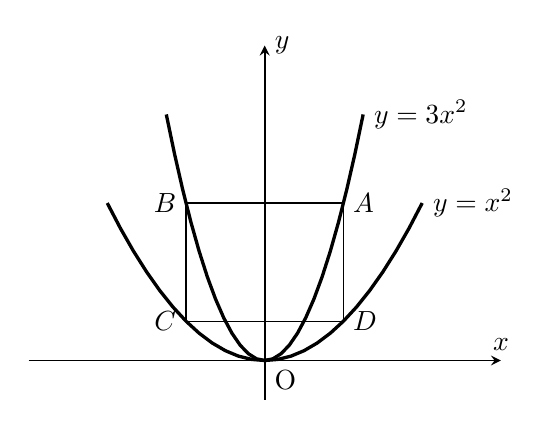
\begin{tikzpicture}[scale=0.5]
		\draw[->,>=stealth,semithick] (-6,0)--(6,0)node[above]{$x$}; %x軸
		\draw[->,>=stealth,semithick] (0,-1)--(0,8)node[right]{$y$}; %y軸
		\draw (0,0)node[below right]{O}; %原点
		\draw(2,4)node[right]{$A$};
		\draw(-2,4)node[left]{$B$};
		\draw(2,1)node[right]{$D$};
		\draw(-2,1)node[left]{$C$};
		\draw(-2,1)rectangle(2,4);
		\draw[very thick,domain=-2.5:2.5] plot(\x, {pow(\x,2)})node[right]{$y=3x^2$};
		\draw[very thick,domain=-4:4] plot(\x, {pow(\x,2)/4})node[right]{$y=x^2$};
	\end{tikzpicture}

\end{itembox}


\begin{itembox}[l]{}
	$y=\frac{1}{3}x-2$上の点Pと$y=-\frac{x^{2}}{3}$上の点Qについて, $PQ=\frac{4}{3}$となるようなPの座標を求めなさい

	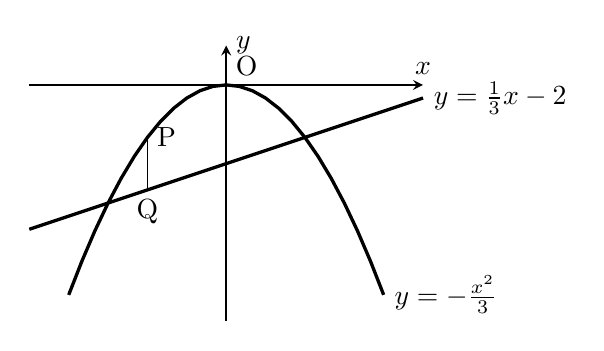
\begin{tikzpicture}[scale=0.5]
		\draw[->,>=stealth,semithick] (-5,0)--(5,0)node[above]{$x$}; %x軸
		\draw[->,>=stealth,semithick] (0,-6)--(0,1)node[right]{$y$}; %y軸
		\draw (0,0)node[above right]{O}; %原点
		\coordinate[label=right:P](P)at(-2,-4/3);
		\coordinate[label=below:Q](Q)at(-2,-8/3);
		\draw(P)--(Q);
		\draw[very thick,domain=-5:5] plot(\x, {\x/3-2})node[right]{$y=\frac{1}{3}x-2$};
		\draw[very thick,domain=-4:4] plot(\x, {-pow(\x,2)/3})node[right]{$y=-\frac{x^{2}}{3}$};
	\end{tikzpicture}
\end{itembox}

\begin{itembox}[l]{}
	$x座標がそれぞれ-2,1であるようなy=x^{2}上の点A,Bについて以下の問いに答えよ$
	\subsubsection{$\triangle PAB =2\triangle OABとなるようなy軸上の点Pの座標を答えよ$}
	\subsubsection{$\triangle QAB =2\triangle OABとなるようなy=x^{2}上の点Qの座標を答えよ$}
	\begin{spacing}{7}
	\end{spacing}
\end{itembox}

\newpage


\section{図形}
\subsection{相似}
\begin{itembox}[l]{三角形の相似条件}
	\begin{Large}
		\begin{itemize}
			\item
			\item
			\item
		\end{itemize}
	\end{Large}
\end{itembox}

\begin{itembox}[l]{比の関係}
	\begin{multicols}{3}
		\begin{itemize}
			\item 相似比  {\Large m:n}
			\item 面積比
			\item 体積比
		\end{itemize}
	\end{multicols}
\end{itembox}

\begin{itembox}[l]{平行線と線分の比}
	\begin{tabular}{cccc}
		\begin{minipage}[t]{0.25\linewidth}
			\begin{tikzpicture}
				\tikz\draw(0,0)--(4,0)--(2,5)--cycle;
				\draw(1,2.5)--(3,2.5);

			\end{tikzpicture}
		\end{minipage}
		\begin{minipage}[t]{0.25\linewidth}
			\begin{tikzpicture}
				\tikz\draw(0,0)--(4,0)--(2,5)--cycle;
				\draw(1,2.5)--(3,2.5);
			\end{tikzpicture}

		\end{minipage}

		\begin{minipage}[t]{0.25\linewidth}
			\begin{tikzpicture}
				\tikz\draw(0,0)--(4,0)--(2,2.5)--cycle;
				\draw(0,5)--(4,5)--(2,2.5)--cycle;

			\end{tikzpicture}

		\end{minipage}


		\begin{minipage}[t]{0.25\linewidth}
			\begin{tikzpicture}
				\draw(0,4)--(4,4);
				\draw(0,2.5)--(4,2.5);
				\draw(0,1)--(4,1);
				\draw(0,0)--(1,5);
				\draw(3,5)--(4,0);
			\end{tikzpicture}

		\end{minipage}
	\end{tabular}

\end{itembox}

\begin{itembox}[l]{中点連結定理}
\vspace{5cm}
\end{itembox}

\begin{itembox}[l]{角の二等分線}
	\begin{tikzpicture}
    %三角形の頂点を設定し,三角形を描く
    \coordinate (O) at (0,0) node [below] at (O) {};
    \coordinate (A) at (5,0) node [below] at (A) {};
    \coordinate (B) at (6,3) node [above right] at (B) {};
    \coordinate (C) at (9,4.5) node [above right] at (C) {};
    \coordinate (D) at (12,0) node [above right] at (D) {};
    \draw (O)--(A)--(B)--cycle;
    \draw[dashed](B)--(C);
    \draw[dashed](A)--(D);
    %各辺上で一定の長さの点を設定する
    \coordinate (s) at ($(O)!1cm!(A)$);
    \coordinate (t) at ($(O)!1cm!(B)$);
    \coordinate (u) at ($(A)!1cm!(O)$);
    \coordinate (v) at ($(A)!1cm!(B)$);
    \coordinate (w) at ($(B)!1cm!(O)$);
    \coordinate (z) at ($(B)!1cm!(A)$);
    \coordinate (c) at ($(B)!1cm!(C)$);
    %内角の二等分線
    \draw [dashed](B)--($(z)!.5!(w)!-4!(B)$) [name path=line B];
    \draw [dashed](B)--($(z)!.5!(c)!-13!(B)$) [name path=line C];
  \end{tikzpicture}
\end{itembox}

\begin{itembox}[l]{比を合わせる}
	一直線上にA, B, C, Dがあるとき、$AB:BD=2:3, AC:CD=3:4$である。$AB:BC:CD$を求めよ
	\\\\\
\end{itembox}



\subsection{円の性質}
\begin{itembox}[l]{}


	\subsubsection*{円周角の定理}
	\begin{multicols}{3}
		\begin{minipage}{0.33\textwidth}
			\begin{tikzpicture}
				\draw(0,0)circle(2.5);
				\fill(0,0)circle(0.06)node[below]{O};
			\end{tikzpicture}

		\end{minipage}
		\begin{minipage}{0.33\textwidth}
			\begin{tikzpicture}
				\draw(0,0)circle(2.5);
				\fill(0,0)circle(0.06)node[below]{O};
			\end{tikzpicture}
		\end{minipage}
		\begin{minipage}{0.33\textwidth}
			\begin{tikzpicture}
				\draw(0,0)circle(2.5);
				\fill(0,0)circle(0.06)node[below]{O};
			\end{tikzpicture}
		\end{minipage}
	\end{multicols}

	\begin{multicols}{2}
		\begin{minipage}{0.5\textwidth}
			\subsubsection*{円に内接する四角形}
			\begin{tikzpicture}
				\draw(0,0)circle(2.5);
				\fill(0,0)circle(0.06)node[below]{O};
			\end{tikzpicture}
		\end{minipage}
		\begin{minipage}{0.5\textwidth}
			\subsubsection*{接弦定理}
			\begin{tikzpicture}
				\draw(0,0)circle(2.5);
				\fill(0,0)circle(0.06)node[below]{O};
			\end{tikzpicture}
		\end{minipage}
	\end{multicols}

\end{itembox}


\subsection{三平方の定理}
\begin{itembox}[l]{三平方の定理}
	辺の長さがそれぞれa,b,cの時、ただしcの長さが一番長い
	\\
\end{itembox}

\begin{itembox}[l]{覚えてほしい直角三角形}
	\begin{multicols}{2}
		\begin{itemize}
			\item 角の大きさが90,60,30
			\item 角の大きさが90,45,45
			\item 全ての辺が整数値(二つ)
		\end{itemize}
	\end{multicols}
\end{itembox}






\end{document}
